\documentclass[aspectratio=169,11pt]{beamer}

% ── Theme ──────────────────────────────────────────────────────────
\usetheme{Madrid}
\usecolortheme{whale}
\setbeamertemplate{navigation symbols}{}
\setbeamertemplate{footline}[frame number]
\setbeamerfont{frametitle}{size=\large,series=\bfseries}

% ── Packages ───────────────────────────────────────────────────────
\usepackage{amsmath,amssymb}
\usepackage{graphicx}
\usepackage{booktabs}
\usepackage{tikz}
\usetikzlibrary{arrows.meta,positioning,shapes.geometric,shapes.misc,calc,decorations.pathreplacing}
\usepackage{xcolor}
\usepackage{appendixnumberbeamer}

% ── Colors ─────────────────────────────────────────────────────────
\definecolor{cA}{RGB}{220,80,60}      % Scheme A — red
\definecolor{cC}{RGB}{50,140,70}      % Scheme C — green
\definecolor{cOracle}{RGB}{40,100,180}% Oracle — blue
\definecolor{cHighlight}{RGB}{230,160,30} % highlight gold
\definecolor{cBg}{RGB}{245,245,250}
\definecolor{cDarkBg}{RGB}{30,55,90}

% ── Math shortcuts ─────────────────────────────────────────────────
\newcommand{\E}{\mathbb{E}}
\newcommand{\R}{\mathbb{R}}
\newcommand{\V}{\mathbb{V}}
\newcommand{\wbar}{\bar{w}}
\newcommand{\what}{\hat{w}}
\newcommand{\wstar}{w^*}
\DeclareMathOperator*{\argmax}{arg\,max}

% ── Meta ───────────────────────────────────────────────────────────
\title[FedProTrack]{Cluster Before You Train\\[4pt]
  \normalsize Fingerprint-Based Concept Discovery\\
  for Federated Learning Under Recurrent Drift}
\author{}
\date{April 2026}
\institute{}

% ===================================================================
\begin{document}

% -------------------------------------------------------------------
\begin{frame}[plain]
\titlepage
\end{frame}

% -------------------------------------------------------------------
\begin{frame}{Outline}
\tableofcontents
\end{frame}

% ===================================================================
\section{Background \& Motivation}
% ===================================================================

% -------------------------------------------------------------------
\begin{frame}{Problem Setting: Federated Learning Under Concept Drift}

\begin{columns}[T]
\begin{column}{0.55\textwidth}
\begin{itemize}
  \item $K$ clients, $T$ rounds, $C$ latent \textbf{concepts}
  \item Each round, client $k$ draws data from concept $c(k,t)\in[C]$
  \item Concepts \textbf{recur}: client may revisit concept $a$ after visiting $b$
  \item Server cannot see raw data --- only aggregated signals
\end{itemize}

\vspace{6pt}
\textbf{Goal}: infer latent concept identity $\to$ group clients $\to$ per-concept federated aggregation

\vspace{6pt}
\textcolor{cOracle}{\textbf{Oracle}} (upper bound): knows true $c(k,t)$ every round
\end{column}

\begin{column}{0.42\textwidth}
\centering
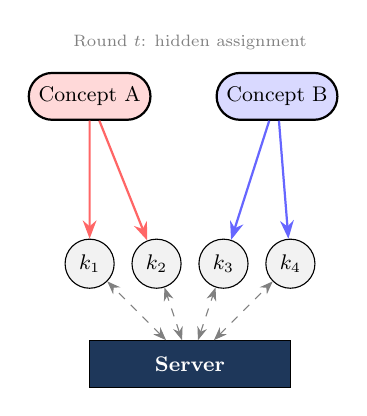
\begin{tikzpicture}[
    client/.style={circle,draw,minimum size=7mm,font=\small},
    concept/.style={rounded rectangle,draw,thick,minimum height=7mm,font=\small},
    >=Stealth, scale=0.85, transform shape
  ]
  % Concepts
  \node[concept,fill=red!15]   (cA) at (0,2.5) {Concept A};
  \node[concept,fill=blue!15]  (cB) at (2.8,2.5) {Concept B};
  % Clients
  \foreach \i/\x in {1/0, 2/1, 3/2, 4/3} {
    \node[client,fill=gray!10] (k\i) at (\x, 0) {$k_{\i}$};
  }
  % Assignments (round t)
  \draw[->,thick,red!60]  (cA) -- (k1);
  \draw[->,thick,red!60]  (cA) -- (k2);
  \draw[->,thick,blue!60] (cB) -- (k3);
  \draw[->,thick,blue!60] (cB) -- (k4);
  % Server
  \node[rectangle,draw,fill=cDarkBg,text=white,minimum width=30mm,minimum height=7mm,font=\small\bfseries] (srv) at (1.5,-1.5) {Server};
  \foreach \i in {1,...,4} {
    \draw[<->,gray,dashed] (srv) -- (k\i);
  }
  % Label
  \node[font=\scriptsize,gray] at (1.5,3.3) {Round $t$: hidden assignment};
\end{tikzpicture}
\end{column}
\end{columns}
\end{frame}

% -------------------------------------------------------------------
\begin{frame}{The Core Design Choice: When to Cluster?}
\centering
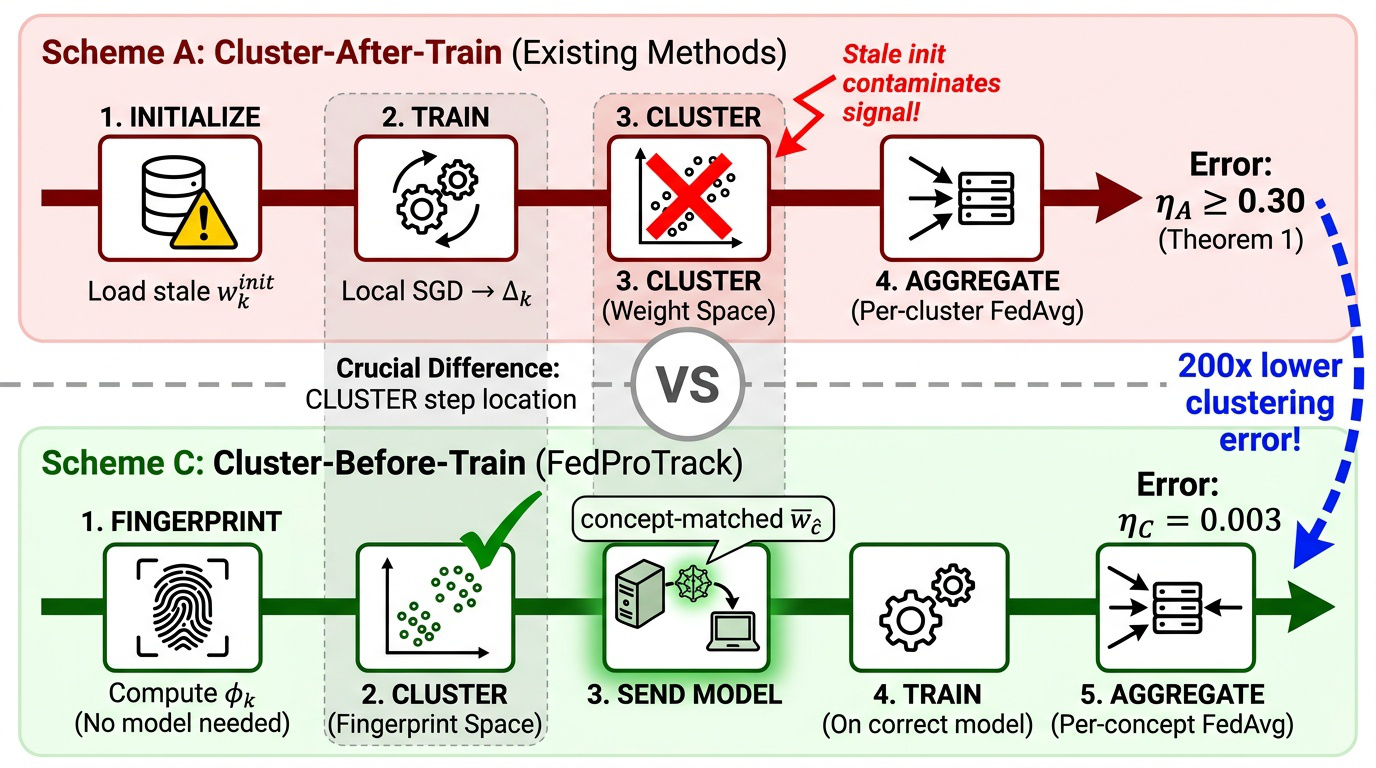
\includegraphics[width=0.82\textwidth]{figures/paperbanana/scheme_comparison_candidate_0.png}

\vspace{1pt}
{\scriptsize
\textbf{Thm 1}: $\eta_A \geq \eta_A^{(\mathrm{clean})} + \kappa \cdot \V(w^{(\mathrm{init})})$ \quad
$\Rightarrow$ \textcolor{cA}{Scheme A: $\eta \geq 0.30$} \quad vs \quad \textcolor{cC}{Scheme C: $\eta = 0.003$}
}
\end{frame}

% ===================================================================
\section{Theoretical Foundation}
% ===================================================================

% -------------------------------------------------------------------
\begin{frame}{When Does Concept-Level Aggregation Help?}
\centering
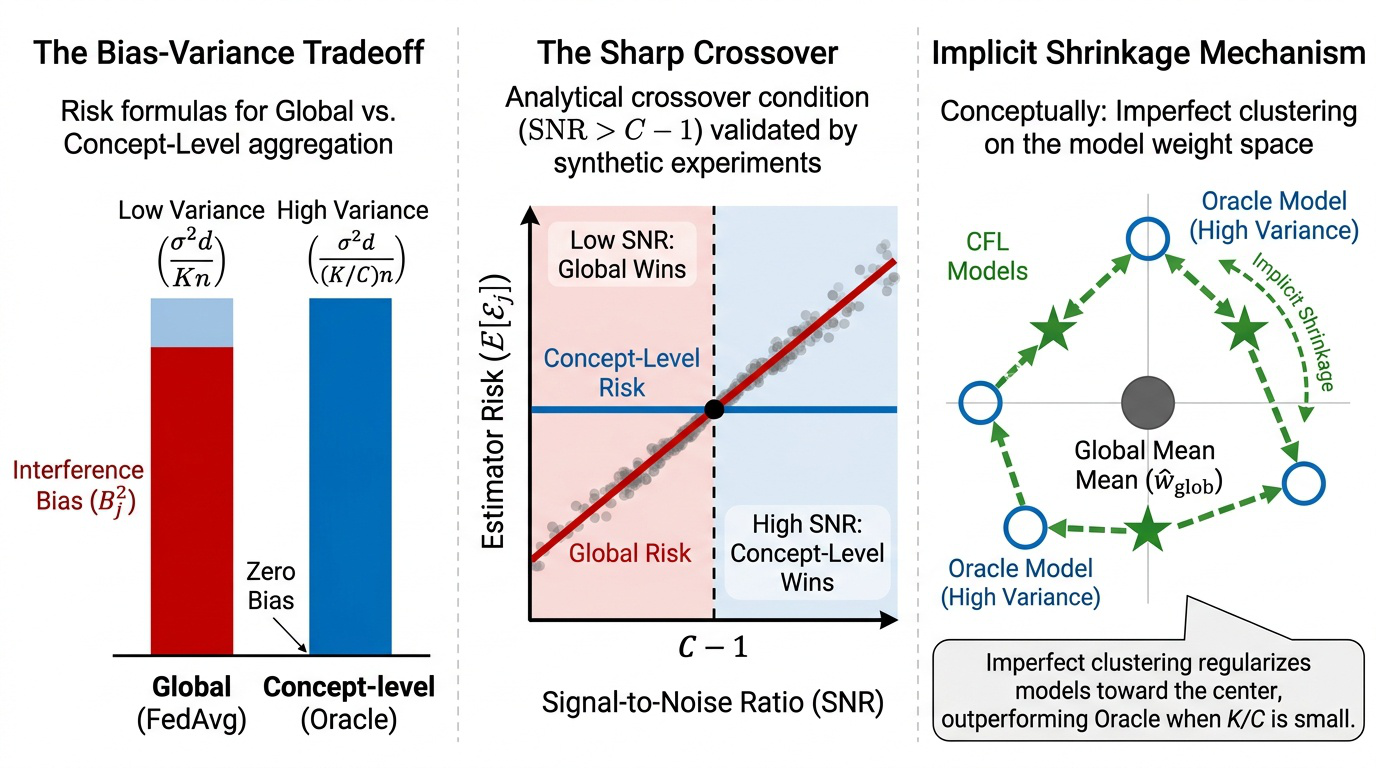
\includegraphics[width=0.78\textwidth]{figures/paperbanana/research_question_candidate_2.png}

\vspace{1pt}
{\scriptsize
\textbf{Left}: Bias-variance tradeoff \quad
\textbf{Center}: Sharp crossover at $\mathrm{SNR} = C{-}1$ \quad
\textbf{Right}: Imperfect clustering $=$ implicit shrinkage
}
\end{frame}

% -------------------------------------------------------------------
\begin{frame}{Existing Methods: Scheme A (Cluster-After-Train)}

\textbf{Nearly all} clustered FL methods follow the same protocol:

\vspace{8pt}
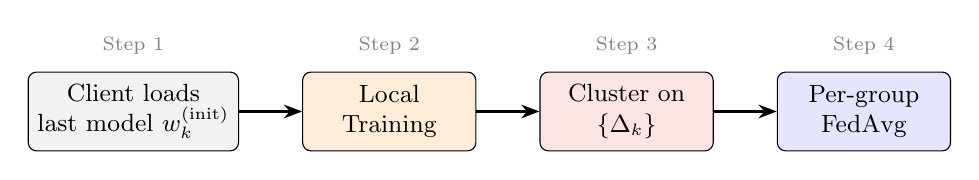
\begin{tikzpicture}[
    box/.style={rectangle,draw,rounded corners=3pt,minimum height=10mm,minimum width=22mm,font=\small,align=center},
    >=Stealth, node distance=8mm
  ]
  \node[box,fill=gray!10] (init) {Client loads\\last model $w_k^{(\mathrm{init})}$};
  \node[box,fill=orange!15,right=of init] (train) {Local\\Training};
  \node[box,fill=cA!15,right=of train] (cluster) {Cluster on\\$\{\Delta_k\}$};
  \node[box,fill=blue!10,right=of cluster] (agg) {Per-group\\FedAvg};
  \draw[->,thick] (init) -- (train);
  \draw[->,thick] (train) -- (cluster);
  \draw[->,thick] (cluster) -- (agg);
  \node[font=\scriptsize,gray,above=1mm of init] {Step 1};
  \node[font=\scriptsize,gray,above=1mm of train] {Step 2};
  \node[font=\scriptsize,gray,above=1mm of cluster] {Step 3};
  \node[font=\scriptsize,gray,above=1mm of agg] {Step 4};
\end{tikzpicture}

\vspace{10pt}
\textbf{Examples}: IFCA, CFL, FedEM, FedRC, FedGWC, gradient-based partitioning \ldots

\vspace{10pt}
\begin{alertblock}{The Hidden Assumption}
The weight update $\Delta_k$ faithfully reflects the client's \emph{current} concept identity.
\end{alertblock}

\vspace{4pt}
\textcolor{cA}{\textbf{But under concept recurrence, this assumption breaks.}}
\end{frame}

% -------------------------------------------------------------------
\begin{frame}{The Stale-Initialisation Problem}

When client switches from concept $a \to b$, it loads a model last trained on $a$:

\begin{equation*}
\Delta_k = \underbrace{-\alpha \nabla L_b(\wbar_b)}_{\text{true concept-}b\text{ signal}}
          + \underbrace{\alpha H_k \bigl(w_k^{(\mathrm{init})} - \wbar_b^{(t-1)}\bigr)}_{\textcolor{cA}{\text{stale-init contamination}}}
          + O(\|\cdot\|^2)
\end{equation*}

\begin{itemize}
  \item The contamination term has \textbf{nothing to do} with concept $b$
  \item It is proportional to $\|w_k^{(\mathrm{init})} - \wbar_b\|$ --- the ``mismatch''
  \item Any clustering algorithm operating on $\Delta_k$ is \textbf{structurally misled}
\end{itemize}

\vspace{4pt}
\centering
\textcolor{cA}{\textbf{$\Rightarrow$ This is not an algorithm problem --- it is a protocol structure problem.}}
\end{frame}

% -------------------------------------------------------------------
\begin{frame}{Theorem: Stale-Initialisation Amplification}

\begin{theorem}[Main Result --- Unconditional]
Under standard regularity conditions (L-smooth, $\mu$-strongly convex):
\begin{equation*}
\boxed{\eta_A \;\geq\; \eta_A^{(\mathrm{clean})} \;+\; \kappa \cdot \V(w^{(\mathrm{init})})}
\end{equation*}
where $\V(w^{(\mathrm{init})}) > 0$ \textbf{whenever concepts recur}.
\end{theorem}

\vspace{6pt}
Three key implications:
\begin{enumerate}
  \item \textbf{Unconditional}: holds under standard assumptions, no extra conditions needed
  \item $\V(w^{(\mathrm{init})}) > 0$ is \textbf{structural} under concept recurrence --- \textbf{cannot be removed}
  \item No algorithm improvement within Scheme A can close this gap
\end{enumerate}

\vspace{6pt}
\textbf{From clustering error to excess risk} (Corollary 1):\\[2pt]
Combining with the implicit-shrinkage characterisation gives excess-risk gap\\
$\geq (\eta_A - \eta_C) \cdot \frac{C}{C-1} \cdot \bar{B}^2 > 0$
\end{frame}

% -------------------------------------------------------------------
\begin{frame}{Empirical Evidence: $\eta \geq 0.30$ For All Scheme A Methods}

\begin{columns}[T]
\begin{column}{0.48\textwidth}
\centering
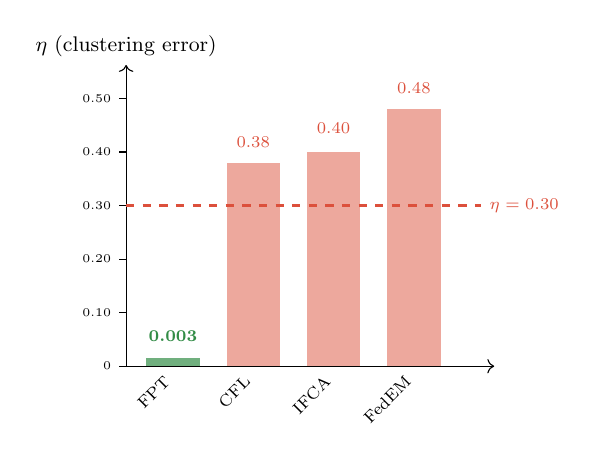
\begin{tikzpicture}[scale=0.85, transform shape]
  % Bar chart: clustering error
  \draw[->] (0,0) -- (0,4.5) node[above,font=\small] {$\eta$ (clustering error)};
  \draw[->] (0,0) -- (5.5,0);
  % bars
  \fill[cC!70] (0.3,0) rectangle (1.1, 0.12);  % FPT
  \fill[cA!50] (1.5,0) rectangle (2.3, 3.04);  % CFL
  \fill[cA!50] (2.7,0) rectangle (3.5, 3.20);  % IFCA
  \fill[cA!50] (3.9,0) rectangle (4.7, 3.84);  % FedEM
  % labels
  \node[font=\scriptsize,rotate=45,anchor=east] at (0.7,-0.1) {FPT};
  \node[font=\scriptsize,rotate=45,anchor=east] at (1.9,-0.1) {CFL};
  \node[font=\scriptsize,rotate=45,anchor=east] at (3.1,-0.1) {IFCA};
  \node[font=\scriptsize,rotate=45,anchor=east] at (4.3,-0.1) {FedEM};
  % values
  \node[font=\scriptsize,cC] at (0.7, 0.45) {\textbf{0.003}};
  \node[font=\scriptsize,cA] at (1.9, 3.35) {0.38};
  \node[font=\scriptsize,cA] at (3.1, 3.55) {0.40};
  \node[font=\scriptsize,cA] at (4.3, 4.15) {0.48};
  % threshold line
  \draw[dashed,thick,cA] (0,2.4) -- (5.3,2.4) node[right,font=\scriptsize] {$\eta = 0.30$};
  % scale
  \foreach \y/\v in {0/0, 0.8/0.10, 1.6/0.20, 2.4/0.30, 3.2/0.40, 4.0/0.50} {
    \draw (0,\y) -- (-0.1,\y) node[left,font=\tiny] {\v};
  }
\end{tikzpicture}
\end{column}

\begin{column}{0.50\textwidth}
\begin{itemize}
  \item On CIFAR-100, \textbf{all} Scheme A methods: $\eta \geq 0.38$
  \item FPT achieves $\eta = 0.003$ --- \textbf{two orders of magnitude lower}
  \item This gap is \emph{structural}, not algorithmic
\end{itemize}

\vspace{8pt}
\textbf{Even with Oracle initialisation} (removing $\V$):\\
$\eta_A^{(\mathrm{clean})} = 0.40$ vs $\eta_C = 0.002$

\vspace{6pt}
$\Rightarrow$ Fingerprints have inherent $d/L$ SNR advantage \\
\quad (Lemma 2: $d=128$, $L=10$ $\Rightarrow$ $12.8\times$)
\end{column}
\end{columns}
\end{frame}

% ===================================================================
\section{Method: FedProTrack}
% ===================================================================

% -------------------------------------------------------------------
\begin{frame}{FedProTrack: Overview}
\centering
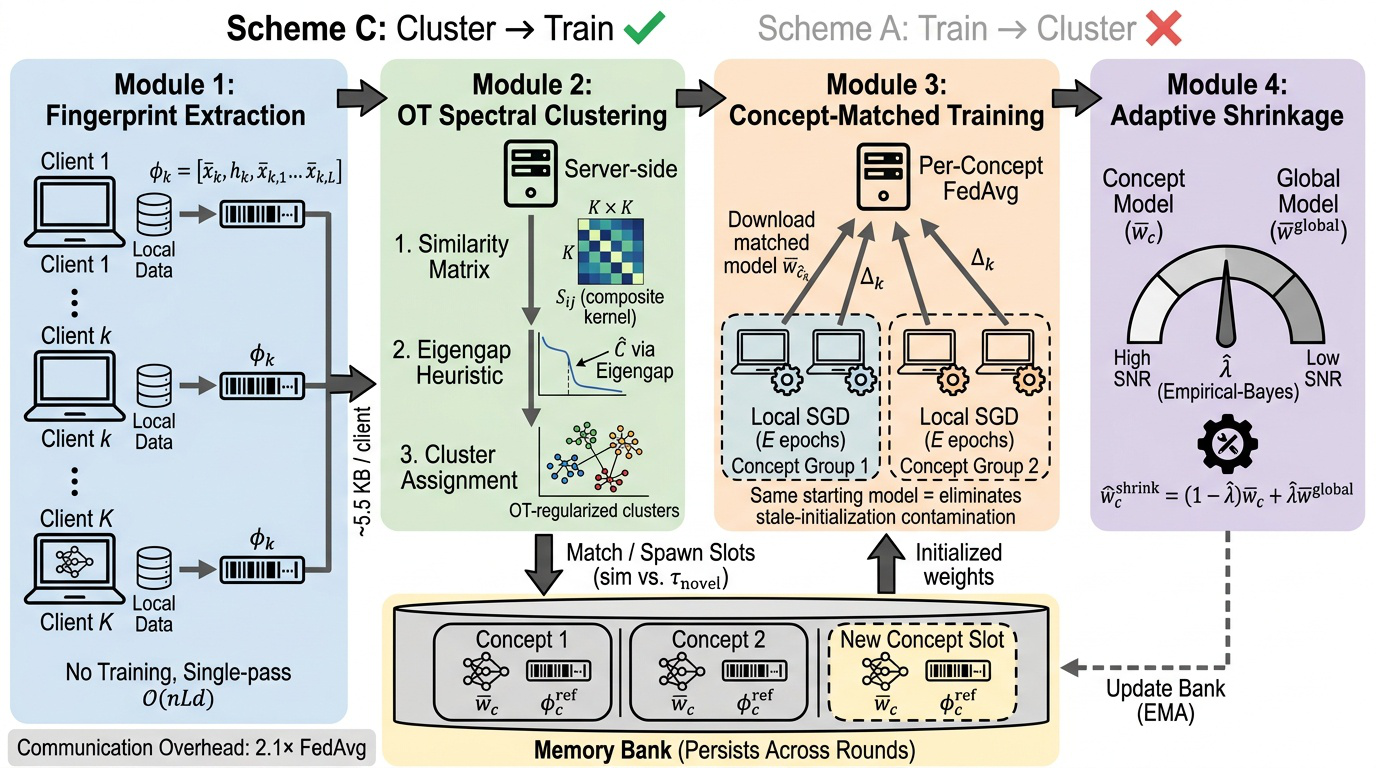
\includegraphics[width=0.78\textwidth]{figures/paperbanana/pipeline_v2_candidate_1.png}

\vspace{1pt}
{\scriptsize
\textbf{Scheme C}: Fingerprint $\to$ OT Spectral Clustering $\to$ Concept-Matched Training $\to$ Adaptive Shrinkage ($2.1\times$ FedAvg)
}
\end{frame}

% -------------------------------------------------------------------
\begin{frame}{Module 1: Fingerprint Extraction}

\small
Each client computes a \textbf{data fingerprint} without any model training:
\vspace{-4pt}
$$\phi_k = \bigl[\underbrace{\bar{x}_k}_{\text{global mean}},\;\;
         \underbrace{h_k}_{\text{label dist.}},\;\;
         \underbrace{\bar{x}_{k,1},\;\ldots,\;\bar{x}_{k,L}}_{\text{class-cond. means}}\bigr]$$

\vspace{-6pt}
\begin{columns}[T]
\begin{column}{0.50\textwidth}
\textbf{Why this design?}
\begin{itemize}\setlength\itemsep{0pt}
  \item Class-conditional means $=$ \textbf{sufficient statistics} for concept identity
  \item Single-pass $O(nLd)$, no gradient needed
  \item $d{=}128$, $L{=}10$ $\Rightarrow$ \textbf{5.5 KB} per client
\end{itemize}
\end{column}

\begin{column}{0.48\textwidth}
\textbf{SNR advantage (Lemma 2):}
\vspace{-6pt}
$$\frac{\mathrm{SNR}_{\mathrm{fp}}}{\mathrm{SNR}_{\mathrm{wt}}} = \frac{d}{L} = \frac{128}{10} = 12.8\times$$
\vspace{-6pt}

Fingerprints encode concept signal as \emph{first-order} moments; weights bury it in \emph{quadratic} forms ($X^\top X$).
\end{column}
\end{columns}
\end{frame}

% -------------------------------------------------------------------
\begin{frame}{Module 2: OT Spectral Clustering --- Step 1: Similarity Matrix}

Given $K$ fingerprints $\{\phi_1, \ldots, \phi_K\}$, the server computes:

\begin{equation*}
S_{ij} = \underbrace{0.25 \cdot \mathrm{sim}_{\mathrm{feat}}(\phi_i, \phi_j)}_{\text{global-mean Gaussian kernel}}
       + \underbrace{0.30 \cdot \mathrm{sim}_{\mathrm{label}}(h_i, h_j)}_{\text{label-histogram cosine}}
       + \underbrace{0.45 \cdot \mathrm{sim}_{\mathrm{cc}}(\phi_i, \phi_j)}_{\text{class-conditional Gaussian kernel}}
\end{equation*}

\vspace{4pt}
\begin{itemize}\setlength\itemsep{2pt}
  \item Weights fixed on held-out synthetic data, \textbf{not tuned} on evaluation
  \item $\mathrm{sim}_{\mathrm{cc}}$ dominates: class-conditional structure carries the most concept signal
  \item \textbf{Robust}: accuracy varies $\leq 0.2$pp across 4 weight configurations
\end{itemize}

\vspace{4pt}
\textbf{Theoretical connection}: for Gaussian classes with shared covariance,
Euclidean distance on class-conditional means $\approx$ \textbf{Wasserstein-2}:
$\;W_2^2(P_a, P_b) = \sum_c w_c \|\mu_a^{(c)} - \mu_b^{(c)}\|^2$
\end{frame}

% -------------------------------------------------------------------
\begin{frame}{Module 2: OT Spectral Clustering --- Step 2: Eigengap}

\textbf{Automatic concept-count selection} via normalised Laplacian:

\begin{columns}[T]
\begin{column}{0.52\textwidth}
\begin{enumerate}
  \item Construct $L_{\mathrm{sym}} = I - D^{-1/2}SD^{-1/2}$
  \item Compute eigenvalues $\lambda_1 \leq \lambda_2 \leq \cdots \leq \lambda_K$
  \item Find the largest gap:
    $$\hat{C} = \argmax_{c \in [2, K/2]} (\lambda_{c+1} - \lambda_c)$$
\end{enumerate}

\vspace{6pt}
\textbf{Intuition}: $C$ well-separated clusters $\Rightarrow$ $C$ eigenvalues $\approx 0$, then a \textbf{jump}

\vspace{6pt}
\textcolor{cC}{\textbf{Result}}: Eigengap correctly recovers $\hat{C}{=}4$ in $>$95\% of rounds. Fixing $\hat{C}{=}C$ costs only 0.6pp.
\end{column}

\begin{column}{0.45\textwidth}
\centering
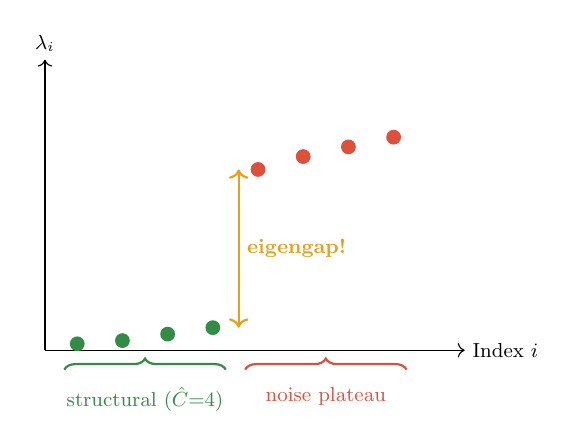
\begin{tikzpicture}[scale=0.82, transform shape]
  % Axes
  \draw[->] (0,0) -- (6.5,0) node[right,font=\small] {Index $i$};
  \draw[->] (0,0) -- (0,4.5) node[above,font=\small] {$\lambda_i$};
  % Eigenvalues
  \filldraw[cC] (0.5, 0.1) circle (3pt);
  \filldraw[cC] (1.2, 0.15) circle (3pt);
  \filldraw[cC] (1.9, 0.25) circle (3pt);
  \filldraw[cC] (2.6, 0.35) circle (3pt);
  % Gap
  \draw[<->,thick,cHighlight] (3.0, 0.35) -- (3.0, 2.8)
    node[midway,right,font=\small\bfseries,text=cHighlight] {eigengap!};
  % Noise plateau
  \filldraw[cA] (3.3, 2.8) circle (3pt);
  \filldraw[cA] (4.0, 3.0) circle (3pt);
  \filldraw[cA] (4.7, 3.15) circle (3pt);
  \filldraw[cA] (5.4, 3.3) circle (3pt);
  % Labels
  \draw[decorate,decoration={brace,amplitude=4pt},thick,cC]
    (0.3,-0.3) -- (2.8,-0.3) node[midway,below=4pt,font=\small,cC] {structural ($\hat{C}{=}4$)};
  \draw[decorate,decoration={brace,amplitude=4pt},thick,cA]
    (3.1,-0.3) -- (5.6,-0.3) node[midway,below=4pt,font=\small,cA] {noise plateau};
\end{tikzpicture}
\end{column}
\end{columns}
\end{frame}

% -------------------------------------------------------------------
\begin{frame}{Module 2: OT Spectral Clustering --- Step 3: OT-Regularised Assignment}
\small
\begin{columns}[T]
\begin{column}{0.55\textwidth}
\textbf{Standard spectral clustering}: top-$\hat{C}$ eigenvectors $\to$ row-normalise $\to$ $k$-means.

\vspace{4pt}
\textbf{Problem}: $k$-means may produce empty/tiny clusters --- a 1-client group has no aggregation benefit.

\vspace{4pt}
\textbf{OT regularisation} replaces $k$-means:
\vspace{-4pt}
$$\min_{\pi} \sum_{i,c} \pi_{ic} \|v_i - \mu_c\|^2$$
\vspace{-10pt}
\begin{align*}
\text{s.t.}\;\; \sum_c \pi_{ic} &= 1 \;\;\forall i \\
\sum_i \pi_{ic} &\geq \lfloor K/(2\hat{C}) \rfloor \;\;\forall c \;\;\textcolor{cC}{\text{(min size)}}
\end{align*}
\end{column}

\begin{column}{0.42\textwidth}
\centering
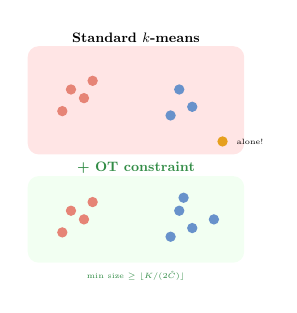
\begin{tikzpicture}[scale=0.55, transform shape]
  % k-means failure
  \node[font=\small\bfseries] at (2.5, 5.2) {Standard $k$-means};
  \fill[red!10,rounded corners] (0,2.5) rectangle (5,5);
  \filldraw[cA!70] (1,4) circle (3pt);
  \filldraw[cA!70] (1.3,3.8) circle (3pt);
  \filldraw[cA!70] (0.8,3.5) circle (3pt);
  \filldraw[cA!70] (1.5,4.2) circle (3pt);
  \filldraw[cOracle!70] (3.5,4) circle (3pt);
  \filldraw[cOracle!70] (3.8,3.6) circle (3pt);
  \filldraw[cOracle!70] (3.3,3.4) circle (3pt);
  \filldraw[cHighlight] (4.5,2.8) circle (3pt);
  \node[font=\tiny,right] at (4.7,2.8) {alone!};
  % OT fix
  \node[font=\small\bfseries,cC] at (2.5, 2.2) {+ OT constraint};
  \fill[green!5,rounded corners] (0,0) rectangle (5,2);
  \filldraw[cA!70] (1,1.2) circle (3pt);
  \filldraw[cA!70] (1.3,1) circle (3pt);
  \filldraw[cA!70] (0.8,0.7) circle (3pt);
  \filldraw[cA!70] (1.5,1.4) circle (3pt);
  \filldraw[cOracle!70] (3.5,1.2) circle (3pt);
  \filldraw[cOracle!70] (3.8,0.8) circle (3pt);
  \filldraw[cOracle!70] (3.3,0.6) circle (3pt);
  \filldraw[cOracle!70] (3.6,1.5) circle (3pt);
  \filldraw[cOracle!70] (4.3,1) circle (3pt);
  \node[font=\tiny,cC] at (2.5,-0.3) {min size $\geq \lfloor K/(2\hat{C})\rfloor$};
\end{tikzpicture}
\end{column}
\end{columns}
\end{frame}

% -------------------------------------------------------------------
\begin{frame}{Module 3: Memory Bank \& Concept Matching}
\small
\begin{columns}[T]
\begin{column}{0.56\textwidth}
Memory bank $\mathcal{M} = \{(\wbar_c, \phi_c^{\mathrm{ref}})\}$ stores model + fingerprint per concept.

\vspace{2pt}
\textbf{Matching}: each new cluster centroid vs stored concepts:
\begin{itemize}\setlength\itemsep{0pt}
  \item $\mathrm{sim} \geq \tau_{\mathrm{novel}}$: \textcolor{cC}{re-identify} $\to$ load stored model
  \item $\mathrm{sim} < \tau_{\mathrm{novel}}$: \textcolor{cHighlight}{new concept} $\to$ fresh slot
\end{itemize}
{\scriptsize $\tau_{\mathrm{novel}}$: 95th percentile of pairwise sim distribution}

\vspace{4pt}
\textbf{Key}: dormant concepts are \emph{recalled}, not re-learned.
\end{column}

\begin{column}{0.42\textwidth}
\centering
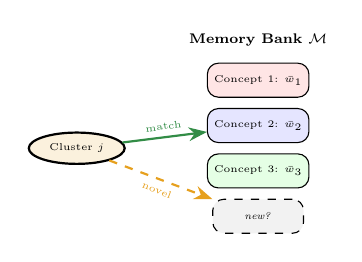
\begin{tikzpicture}[
    slot/.style={rectangle,draw,rounded corners,minimum width=16mm,minimum height=6mm,font=\tiny},
    >=Stealth, scale=0.72, transform shape
  ]
  \node[font=\scriptsize\bfseries] at (2,3.8) {Memory Bank $\mathcal{M}$};
  \node[slot,fill=red!10]   (s1) at (2,3.1) {Concept 1: $\wbar_1$};
  \node[slot,fill=blue!10]  (s2) at (2,2.3) {Concept 2: $\wbar_2$};
  \node[slot,fill=green!10] (s3) at (2,1.5) {Concept 3: $\wbar_3$};
  \node[slot,fill=gray!10,dashed]  (s4) at (2,0.7) {\textit{new?}};

  \node[ellipse,draw,thick,fill=cHighlight!15,font=\tiny] (cl) at (-1.2,1.9) {Cluster $j$};
  \draw[->,thick,cC] (cl) -- (s2) node[midway,above,font=\tiny,sloped] {match};
  \draw[->,thick,dashed,cHighlight] (cl) -- (s4) node[midway,below,font=\tiny,sloped] {novel};
\end{tikzpicture}
\end{column}
\end{columns}
\end{frame}

% -------------------------------------------------------------------
\begin{frame}{Module 4: Concept-Matched Training \& Adaptive Shrinkage}

\begin{columns}[T]
\begin{column}{0.48\textwidth}
\textbf{Concept-Matched Training}

Client $k$ in concept $\hat{c}_k$ receives $\wbar_{\hat{c}_k}^{(t-1)}$ from memory:
\vspace{-2pt}
$$\Delta_k^{(t)} = w_k^{(t)} - \wbar_{\hat{c}_k}^{(t-1)}$$
\vspace{-8pt}
$$\wbar_c^{(t)} = \wbar_c^{(t-1)} + \frac{1}{|\mathcal{C}_c|}\sum_{k\in\mathcal{C}_c}\Delta_k^{(t)}$$

\vspace{-2pt}
{\small All clients in $\mathcal{C}_c$ start from the \textbf{same} model $\Rightarrow$ \textbf{pure concept signal}, no stale-init.}
\end{column}

\begin{column}{0.48\textwidth}
\textbf{Adaptive Shrinkage}
\vspace{-2pt}
$$\what_c^{\mathrm{shrink}} = (1{-}\hat\lambda)\wbar_c^{(t)} + \hat\lambda\,\wbar^{(t)}$$
\vspace{-8pt}
$$\hat\lambda = \frac{\hat\sigma^2/((K/\hat{C})n)}{\hat\sigma^2/((K/\hat{C})n) + \hat\sigma_B^2}$$

\vspace{-2pt}
\begin{itemize}\setlength\itemsep{1pt}
  \item \textbf{High SNR}: $\hat\lambda \to 0$, fully concept-specific
  \item \textbf{Low SNR}: $\hat\lambda \to 1$, degrades to FedAvg
\end{itemize}
\end{column}
\end{columns}

\vspace{4pt}
\centering
\textcolor{cC}{\textbf{Safety net}}: even if clustering is noisy or SNR is low, FPT never hurts much.
\end{frame}

% ===================================================================
\section{Experiments}
% ===================================================================

% -------------------------------------------------------------------
\begin{frame}{Experimental Setup}

\begin{columns}[T]
\begin{column}{0.48\textwidth}
\textbf{4 Datasets}:
\begin{itemize}
  \item \textbf{CIFAR-100} (flagship, 5 configs)
  \item \textbf{Fashion-MNIST}
  \item \textbf{fMoW} (natural temporal drift)
  \item \textbf{CIFAR-10} (negative control)
\end{itemize}

\vspace{6pt}
$K{=}20$, $T{=}100$, $C{=}4$, recurrence period $\rho{=}25$

\vspace{4pt}
Frozen ResNet-18 features, PCA to $d{=}128$\\
Linear classifier (1290 params)\\
\textbf{Identical budgets}: 5 epochs, lr=0.01
\end{column}

\begin{column}{0.48\textwidth}
\textbf{26 Baselines from 7 Families}:
\begin{itemize}
  \item \textcolor{cA}{Cluster-after-train}: IFCA, CFL, FedEM, FedRC
  \item Cluster-late: HCFL, FedGWC
  \item Drift-aware: FedDrift, Flash, FedCCFA
  \item Personalized: FedProx, APFL, Ditto, pFedMe
  \item Core: FedAvg, Oracle, LocalOnly
  \item Misc: FLUX, SCAFFOLD, \ldots
\end{itemize}

\vspace{6pt}
Each baseline uses \textbf{published defaults}; grid-search on held-out config.
\end{column}
\end{columns}
\end{frame}

% -------------------------------------------------------------------
\begin{frame}{Main Results}

\centering
{\small
\setlength{\tabcolsep}{5pt}
\begin{tabular}{@{}l cccc c@{}}
\toprule
& \multicolumn{4}{c}{\textbf{Accuracy} ($\uparrow$)} & \textbf{Clust.~Err.} \\
\cmidrule(lr){2-5} \cmidrule(l){6-6}
Method & CIFAR-100 & F-MNIST & fMoW & CIFAR-10 & $\eta$ (C-100) \\
\midrule
\textcolor{cOracle}{Oracle} & .673 & .974 & .599 & .940 & .000 \\
FedAvg & .631 & .912 & .506 & .917 & --- \\
\midrule
\textcolor{cA}{CFL} & .623 & .922 & .507 & .916 & \textcolor{cA}{.38} \\
\textcolor{cA}{IFCA} & .599 & .821 & .502 & .713 & \textcolor{cA}{.40} \\
\textcolor{cA}{FedEM} & .523 & .866 & .416 & .857 & \textcolor{cA}{.48} \\
\midrule
APFL & .640 & .924 & .515 & .905 & --- \\
Flash & .635 & .920 & .508 & .917 & --- \\
\midrule
\textcolor{cC}{\textbf{FPT (Ours)}} & \textcolor{cC}{\textbf{.670}} & \textcolor{cC}{\textbf{.973}} & \textcolor{cC}{\textbf{.584}} & .907 & \textcolor{cC}{\textbf{.003}} \\
\midrule
Oracle gap (pp) & 4.7 & 6.1 & 9.3 & 2.3 & \\
\textbf{Gap closed} & \textbf{93\%} & \textbf{98\%} & \textbf{84\%} & $-43\%$ & \\
\bottomrule
\end{tabular}
}

\vspace{2pt}
{\small
\textcolor{cC}{\textbf{FPT closes 84--98\% of Oracle gap}} (gap $>$ 4pp) \quad|\quad
\textcolor{cA}{All Scheme A: $\eta \geq 0.38$, below FedAvg} \quad|\quad
CIFAR-10 (neg.~ctrl): FPT degrades gracefully
}
\end{frame}

% -------------------------------------------------------------------
\begin{frame}{Ablation: Every Module Matters}

\centering
{\small
\begin{tabular}{@{}lcc@{}}
\toprule
Variant & Accuracy & $\eta$ \\
\midrule
FPT (full) & $.716 \pm .031$ & $.003 \pm .001$ \\
\quad $-$ Concept discovery & $.684 \pm .028$ & --- \\
\quad $-$ Adaptive shrinkage & $.704 \pm .033$ & $.003 \pm .001$ \\
\quad $-$ Fingerprint $\to$ weights \textcolor{cA}{(Scheme A)} & $.688 \pm .035$ & \textcolor{cA}{$.39 \pm .04$} \\
\quad $-$ Eigengap (fixed $\hat{C} {=} C$) & $.710 \pm .030$ & $.004 \pm .001$ \\
\bottomrule
\end{tabular}
}

\vspace{2pt}
\begin{columns}[T]
\begin{column}{0.48\textwidth}
\textbf{Key row}: fingerprint $\to$ weight-space clustering\\
$\eta$: $0.003 \to 0.39$, Acc: $0.716 \to 0.688$\\[2pt]
\textcolor{cA}{$\Rightarrow$ Isolates the \textbf{protocol ordering effect}}
\end{column}
\begin{column}{0.48\textwidth}
\begin{itemize}\setlength\itemsep{0pt}
  \item $-$ concept discovery: $-3.2$pp
  \item $-$ shrinkage: $-1.2$pp
  \item $-$ eigengap: $-0.6$pp (reliable)
\end{itemize}
\end{column}
\end{columns}
\end{frame}

% -------------------------------------------------------------------
\begin{frame}{Additional Analysis}

\begin{columns}[T]
\begin{column}{0.48\textwidth}
\textbf{$K$-Scaling}
\begin{itemize}
  \item CFL matches Oracle at $K{=}4$ (implicit shrinkage helps when $K/C$ is small)
  \item CFL falls behind by 3.7pp at $K{=}20$
  \item FPT: $\eta \leq 0.01$ at \textbf{all} $K$ values
  \item Confirms Corollary 1 (implicit shrinkage)
\end{itemize}

\vspace{8pt}
\textbf{Communication Cost}
\begin{itemize}
  \item FPT: $2.1\times$ FedAvg per round
  \item Fingerprint: 5.5 KB upload
  \item Server clustering: $<1$ms ($K{=}20$)
  \item Delivers +3.0--6.9pp over best $1\times$ baseline
\end{itemize}
\end{column}

\begin{column}{0.48\textwidth}
\textbf{Boundary Conditions}
\begin{itemize}
  \item \textbf{No recurrence} ($\rho{=}15, T{=}30$):\\
    FPT $\approx$ FedAvg within $-0.1$pp\\
    ($\hat\lambda \to 1$, shrinkage dominates)
  \item \textbf{End-to-end CNN} (EMNIST):\\
    FPT achieves 89--90\% (mid-pack)\\
    Feature drift breaks fingerprints
\end{itemize}

\vspace{8pt}
\textbf{Weight Sensitivity}
\begin{itemize}
  \item Kernel weights $(\alpha_1, \alpha_2, \alpha_3)$:\\
    4 configurations tested
  \item Accuracy varies $\leq 0.2$pp
  \item $\eta_C$ unchanged
\end{itemize}
\end{column}
\end{columns}
\end{frame}

% ===================================================================
\section{Conclusion}
% ===================================================================

% -------------------------------------------------------------------
\begin{frame}{Limitations}

\begin{enumerate}\setlength\itemsep{4pt}
  \item \textbf{Frozen-backbone assumption} ---
    FPT relies on stable feature representations; end-to-end training breaks cross-round fingerprint comparability (EMNIST: mid-pack)

  \item \textbf{Gaussian linear model for theory} ---
    Theorem 1 proven under L-smooth, strongly-convex losses; non-convex extension is future work

  \item \textbf{Scale} ---
    Experiments use $K \leq 40$; spectral clustering is $O(K^3)$, scaling to $K > 1000$ needs Nystr\"{o}m approximation

  \item \textbf{Privacy} ---
    Fingerprints are aggregate statistics (not raw data), but formal DP analysis is beyond scope
\end{enumerate}
\end{frame}

% -------------------------------------------------------------------
\begin{frame}{Takeaways}

\begin{enumerate}\setlength\itemsep{4pt}
  \item \textbf{``When to cluster'' is a critical design dimension}\\
    Scheme A suffers from \textbf{unconditional} stale-init amplification --- protocol-level, not algorithmic

  \item \textbf{Data fingerprints $>$ weight updates for concept discovery}\\
    $d/L$ SNR advantage: $\eta_C = 0.003$ vs $\eta_A \geq 0.38$ (two orders of magnitude)

  \item \textbf{FedProTrack: a complete Scheme C instantiation}\\
    OT spectral clustering + concept memory + adaptive shrinkage $=$ \textbf{84--98\% Oracle gap closed} across 4 datasets, 26 baselines ($2.1\times$ FedAvg communication)

  \item \textbf{Adaptive shrinkage = safety net}\\
    Graceful degradation to FedAvg when concept structure is weak
\end{enumerate}
\end{frame}

\end{document}
